\documentclass[tikz,border=10pt]{standalone}
\usetikzlibrary{positioning, arrows.meta, calc, patterns, backgrounds, babel}
\usepackage[utf8]{inputenc}
\usepackage[T1]{fontenc}
\usepackage{lmodern}
\usepackage[english]{babel}
\usepackage{amsmath, amssymb, bm}

\begin{document}
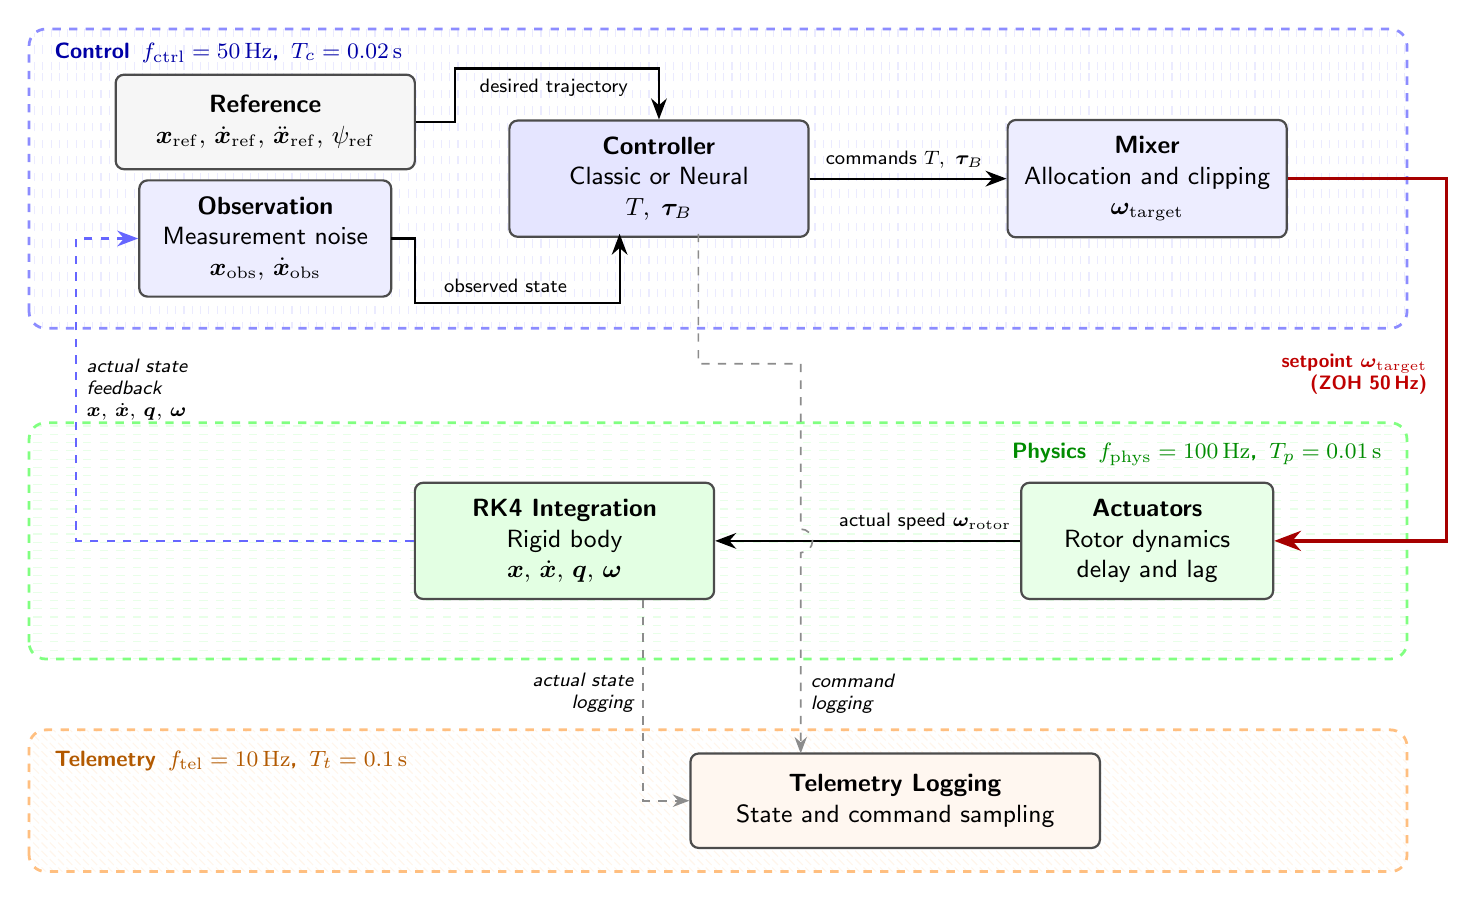
\begin{tikzpicture}[
  align=center,
  font=\sffamily\small,
  box/.style={
    draw=black!70, rectangle, rounded corners=3pt,
    minimum width=3.2cm, minimum height=1.2cm,
    thick, fill=white, inner sep=6pt
  },
  widebox/.style={box, minimum width=3.8cm},
  arr/.style ={draw, -{Stealth[scale=1.15]}, thick},
  darr/.style={draw, -{Stealth[scale=1.15]}, thick, dashed, draw=blue!60},
  tarr/.style={draw, -{Stealth[scale=1.05]}, semithick, dashed, draw=black!45},
]

\def\xBL{-9.0}   \def\xBR{8.5}
\def\yC{0}     \def\hC{1.90}
\def\yF{-4.60} \def\hF{1.50}
\def\yT{-7.90} \def\hT{0.90}
\def\xZOH{9.0}
\def\xFB{-8.4}

%% ====================================================================
%%  BACKGROUND BANDS
%% ====================================================================
\begin{scope}[on background layer]
  \filldraw[draw=blue!45, fill=blue!3,
            pattern=vertical lines, pattern color=blue!8,
            rounded corners=6pt, dashed, line width=1pt]
    (\xBL,\yC-\hC) rectangle (\xBR,\yC+\hC);

  \filldraw[draw=green!50, fill=green!3,
            pattern=horizontal lines, pattern color=green!9,
            rounded corners=6pt, dashed, line width=1pt]
    (\xBL,\yF-\hF) rectangle (\xBR,\yF+\hF);

  \filldraw[draw=orange!50, fill=orange!3,
            pattern=north west lines, pattern color=orange!8,
            rounded corners=6pt, dashed, line width=1pt]
    (\xBL,\yT-\hT) rectangle (\xBR,\yT+\hT);
\end{scope}

%% ====================================================================
%%  BAND LABELS
%% ====================================================================
\node[anchor=north west, font=\sffamily\footnotesize\bfseries, text=blue!65!black]
  at (\xBL+0.20, \yC+\hC-0.05)
  {Control\enspace $f_{\mathrm{ctrl}}=50\,\mathrm{Hz}$,\enspace $T_c=0.02\,\mathrm{s}$};

\node[anchor=north east, font=\sffamily\footnotesize\bfseries, text=green!55!black]
  at (\xBR-0.20, \yF+\hF-0.14)
  {Physics\enspace $f_{\mathrm{phys}}=100\,\mathrm{Hz}$,\enspace $T_p=0.01\,\mathrm{s}$};

\node[anchor=north west, font=\sffamily\footnotesize\bfseries, text=orange!70!black]
  at (\xBL+0.20, \yT+\hT-0.14)
  {Telemetry\enspace $f_{\mathrm{tel}}=10\,\mathrm{Hz}$,\enspace $T_t=0.1\,\mathrm{s}$};

%% ====================================================================
%%  BLOCKS -- CONTROL BAND
%% ====================================================================
\node[widebox, fill=gray!7] (ref) at (-6.0, \yC+0.72) {
  \textbf{Reference}\\
  $\bm{x}_{\mathrm{ref}},\,\dot{\bm{x}}_{\mathrm{ref}},\,\ddot{\bm{x}}_{\mathrm{ref}},\,\psi_{\mathrm{ref}}$
};

\node[box, fill=blue!7] (obs) at (-6.0, \yC-0.76) {
  \textbf{Observation}\\
  Measurement noise\\
  $\bm{x}_{\mathrm{obs}},\,\dot{\bm{x}}_{\mathrm{obs}}$
};

\node[widebox, fill=blue!10] (ctrl) at (-1.0, \yC) {
  \textbf{Controller}\\
  Classic or Neural\\
  $T,\;\bm{\tau}_B$
};

\node[box, fill=blue!7] (mix) at (5.2, \yC) {
  \textbf{Mixer}\\
  Allocation and clipping\\
  $\bm{\omega}_{\mathrm{target}}$
};

%% -- Control arrows --
\draw[arr] (ref.east) -- ([xshift=0.5cm]ref.east) |- node[below, font=\sffamily\scriptsize, pos=0.75]{desired trajectory} (-1.0, 1.4) -- (ctrl.north);
\draw[arr] (-4.4, -0.76) -- (-4.1, -0.76) |- node[above, font=\sffamily\scriptsize, pos=0.73]{observed state} (-1.5, -1.58) -- (-1.5, -0.7);
\draw[arr] (ctrl.east) -- node[above, font=\sffamily\scriptsize]{commands $T,\;\bm{\tau}_B$} (mix.west);

%% ====================================================================
%%  BLOCKS -- PHYSICS BAND
%% ====================================================================
\node[box, fill=green!9] (act) at (5.2, \yF) {
  \textbf{Actuators}\\
  Rotor dynamics\\
  delay and lag
};

\node[widebox, fill=green!11] (rk4) at (-2.2, \yF) {
  \textbf{RK4 Integration}\\
  Rigid body\\
  $\bm{x},\,\dot{\bm{x}},\,\bm{q},\,\bm{\omega}$
};

\draw[arr] (act.west) -- node[above, font=\sffamily\scriptsize, pos=0.30]{actual speed $\bm{\omega}_{\mathrm{rotor}}$} (rk4.east);

%% ====================================================================
%%  BLOCK -- TELEMETRY BAND
%% ====================================================================
\node[widebox, minimum width=5.2cm, fill=orange!6] (tel) at (2.0, \yT) {
  \textbf{Telemetry Logging}\\
  State and command sampling
};

%% ====================================================================
%%  RIGHT CHANNEL (ZOH): Mixer -> Actuators
%% ====================================================================
\draw[arr, draw=red!65!black, line width=1.2pt]
  (mix.east) -- (\xZOH, \yC)
  -- node[left, pos=0.54, xshift=-3pt, font=\sffamily\scriptsize\bfseries, text=red!75!black, align=right]
       {setpoint $\bm{\omega}_{\mathrm{target}}$\\(ZOH 50\,Hz)}
     (\xZOH, \yF)
  -- (act.east);

%% ====================================================================
%%  LEFT CHANNEL (FB): RK4 -> Observation (Feedback)
%% ====================================================================
\draw[darr]
  (rk4.west) -- (\xFB, \yF)
  -- node[right, font=\sffamily\scriptsize\itshape, align=left]
       {actual state\\feedback\\$\bm{x},\,\dot{\bm{x}},\,\bm{q},\,\bm{\omega}$}
     (\xFB, \yC-0.76)
  -- (obs.west);

%% ====================================================================
%%  TELEMETRY 1: RK4 -> Logging (Actual State)
%% ====================================================================
\draw[tarr]
  ([xshift=1.0cm]rk4.south) |- node[left, font=\sffamily\scriptsize\itshape, pos=0.23, align=right] {actual state\\logging}
  (tel.west);

%% ====================================================================
%%  TELEMETRY 2: Controller -> Logging (Commands)
%% ====================================================================
\draw[tarr]
  (-0.5, -0.7) -- (-0.5, -2.35)
  -- (0.8, -2.35)
  -- (0.8, -4.45)
  arc[start angle=90, end angle=-90, radius=0.15]
  -- (0.8, -7.3)
  node[right, font=\sffamily\scriptsize\itshape, pos=0.7, align=left] {command\\logging};

\end{tikzpicture}
\end{document}
